\documentclass[11pt]{article}
\usepackage[a4paper,margin=1in]{geometry}
\usepackage{amsmath,amssymb,mathtools}
\usepackage{graphicx}
\usepackage{booktabs}
\usepackage{longtable}
\usepackage{array}
\usepackage[T1]{fontenc}
\usepackage{lmodern}
\usepackage{microtype}
\usepackage[hidelinks]{hyperref}
\usepackage{enumitem}
\setlist{nosep,leftmargin=1.4em}
\setlength{\emergencystretch}{1.5em}
\newcommand{\G}{\Gamma}
% permit line breaks after underscores inside long identifiers
\let\origunderscore\_
\renewcommand{\_}{\origunderscore\allowbreak}
\newcommand{\W}{3+2\sqrt{2}}
\title{\textsc{One Body}\\A common reflection coordinate, four developments,\\and a table that cannot select its own constant}
\author{Jeromie Beasley\\[3pt]
{\small with GPT (OpenAI), Claude (Anthropic), Grok (xAI), and Open Math}%
\thanks{The research questions, direction and judgements are the author's. GPT, Claude, Grok and
Open Math were used to search the literature, write and check code and Lean proofs, recompute the
archive counts, and draft and referee the text. No statement rests on a model's say-so: every
proved claim is kernel-checked and axiom-audited, and every measured claim is reproduced by a
named script listed in Appendix~\ref{app:ledger}.}}
\date{23 November 2026}

\begin{document}
\maketitle

\begin{abstract}
\noindent
Four separately published or separately written bodies of work by the same author---a periodic
table read as chains of removal energies, a loop wall in a reflection coordinate, a theory of
predictive states and their clock, and a treatment of Ramanujan's gamma fractions as stacks of
faces---are usually described as related. This paper says exactly how, and no more. All four are
written in one small coordinate: a positive ratio $z$, the reflection
$\G=(z-1)/(z+1)=\tanh(\tfrac12\log z)$, the value $\G^2=\tfrac12$, and the rule that reflections
compose by adding their rapidities. Three interfaces between them are compiled rather than
asserted.

Two consequences are not in the individual papers. A window of peel steps can cross the wall with
every one of its steps inside it, because reflections add; in the shipped archive $91{,}638$ of
$91{,}768$ crossing windows are of that kind, while no window crosses on geometric mean. And the
archive cannot select the value $\W$: every cutoff in an interval around it classifies all
$3{,}570$ steps identically, and the aggregate counts that look like confirmation are computed
from the cutoff rather than measuring it.

The contribution is therefore a checked artifact and a set of limits: about $1{,}600$ named
results in one build, three compiled interfaces, a corrigenda list of statements that turned out
false, and a computation showing what the evidence does not establish. No physical mechanism is
derived and no predictive power over chemistry is claimed.
\end{abstract}

\section{Introduction}

The papers this one draws on were written separately and each has its own scope statements.
Reading them together, one notices the same three lines of algebra in all of them: a ratio turned
into a reflection, a distinguished value of that reflection, and an addition law. The temptation
is to call that an identification. It is not. What is true is narrower and can be stated exactly:
the developments share a coordinate, and three of the interfaces between them are compiled---the
two predictive quotients are proved to be the same subspace, one development's path-descent
theorem is specialised to another's ledger, and two peel steps are proved to compose by the
velocity law.

Everything else is a reading. The continued fraction's terms being these faces is a reading, and
the knot involution being an instance of the generic oddness lemma is a reading. Section~\ref{sec:where}
says which is which, sentence by sentence, and Section~\ref{sec:scope} says what is consequently
not claimed.

The paper makes two further points of substance. Section~\ref{sec:data} shows that the data layer
is almost entirely a story about composition, and Section~\ref{sec:band} shows that the same data
cannot select the constant the composition story is organized around. The second is the more
defensible result and the less welcome one.

\section{The coordinate}

\subsection{Ratio and reflection}

Take a ladder of positive readings $I_1,I_2,\dots$---removal energies of one atom, or any other
ordered positive sequence. A step is $z=I_{k+1}/I_k$, and its reflection is
\begin{equation}
\G=\frac{z-1}{z+1}=\tanh\!\Big(\tfrac12\log z\Big). \label{eq:smith}
\end{equation}
The identity is the logarithmic form of $\operatorname{artanh}$ (DLMF 4.37.24); the inverse
$z=(1+\G)/(1-\G)$ is the Cayley coordinate. Reversal sends $z\mapsto 1/z$ and $\G\mapsto-\G$, so
$\G^2$ is reversal-invariant and $\G$ is the only reversal-odd part of the datum.
(Proved: \texttt{LoopWall/Ledger.lean}, \texttt{gam\_eq\_tanh\_half\_log},
\texttt{gam\_reverse}, \texttt{gam\_sq\_reverse}; a second independent proof of
\eqref{eq:smith} is \texttt{unified/VOTKP/Smith.lean}, \texttt{smith\_identity}.)

\subsection{The wall}

One value is distinguished: $\G^2=\tfrac12$. Over positive ratios it is exactly
\begin{equation}
z=\W=5.828427\ldots \quad\text{or its reciprocal}\quad 3-2\sqrt2,
\end{equation}
and in ledger units, where $r=\log z$ is the rapidity, the wall is $r=\pm 2\log(1+\sqrt2)$.
(Proved: \texttt{LoopWall/Wall.lean}, \texttt{wall\_eq\_iff};
\texttt{unified/Bridge/Reflection.lean}, \texttt{wall\_ledger\_value}.)

The name is a definition. In the lossless two-channel normalisation the reflected and transmitted
shares are $\G^2$ and $1-\G^2$, and at $\G^2=\tfrac12$ they coincide; nothing here fixes whether
$\G$ is an amplitude or a power. What gives the value weight is that it keeps marking where a sum
of steps changes qualitative behaviour.

\subsection{Composition}

Rapidities add. A window of steps has ratio the product of its ratios, and in the reflection
coordinate this is the velocity-addition law
\begin{equation}
\G(z_1z_2)=\G(z_1)\oplus\G(z_2),\qquad u\oplus v=\frac{u+v}{1+uv}, \label{eq:oplus}
\end{equation}
which is DLMF 4.35.3 in the tangent-half-angle variable. Hence:
\begin{enumerate}[label=(\alph*)]
\item a window exceeds the upper wall $\W$ exactly when the sum of its steps' rapidities exceeds
  $\log\W$; no single step need cross;
\item the geometric mean of steps that are each inside the wall is inside the wall, for any
  positive ladder, because a mean is bounded by its largest term.
\end{enumerate}
(Proved: \texttt{unified/Bridge/Composition.lean}---\texttt{composite\_reflection\_eq},
\texttt{composite\_two\_eq\_oplus}, \texttt{crosses\_iff\_ledger\_sum}, \texttt{two\_halves\_cross},
\texttt{geomean\_lt\_wall}, \texttt{composition\_crosses\_mean\_does\_not}.)

Statement (a) is the application to a ladder of the elementary fact that a product exceeds a
threshold exactly when the sum of logarithms does (DLMF 4.8.2 with monotonicity); statement (b) is
the equally elementary bound on a mean. Neither is a new criterion, and Section~\ref{sec:prior}
does not claim one. What is new is that they are the right way to read the data.

\section{Where it applies}\label{sec:where}

\subsection{Elemental peeling}

Read an element as the ladder of its successive ionisation energies. The shipped archive has 118
elements and $5{,}714$ steps, of which the hydrogen-to-astatine baseline is 85 elements and
$3{,}570$ steps. Eight of the baseline steps lie outside the wall, and every one is the first
opening of a noble-gas core: Li at $k=1$, Be at 2, B at 3, C at 4 (helium); Na at 1 (neon); K at 1
(argon); Rb at 1 (krypton); Cs at 1 (xenon). Sixty-five further ``anion rungs''---the ratio from
the electron affinity to the first ionisation energy---give 53 more values outside.
(Measured: \texttt{scripts/atlas\_census.py}.)

That is exact arithmetic. As an explanation it is a restatement: a core opening costs much more
than the removal that follows, which is what ``core opening'' means.

\subsection{Dirac time}

The predictive quotient---the state space modulo everything no future reading can see---is the
finite-dimensional observability quotient of linear systems theory: the unobservable subspace is
the intersection of the kernels of $RL^n$, the quotient is by it, and its dimension is the rank of
the observability map. Two developments prove this independently, and the two versions are the
same subspace, Cayley--Hamilton being the bridge. (Proved: \texttt{unified/Bridge/Quotient.lean},
\texttt{unseen\_eq\_unobservable}.)

The same work gives the gap law $\mu_j-\mu_k=\dot\tau(E_j-E_k)$ for a generator with eigen-data
(proved: \texttt{unified/DiracTime/CommonClock.lean}, \texttt{common\_gap\_scaling}). Read as a
peel rate this says the frequency of the peel flow is the clock rate times the energy gap. For a
real gap $\delta$ and the zero-offset flow $\G(\tau)=\tanh(\delta\tau/2)$, the squared wall has
exactly one forward solution precisely when $\delta$ is nonzero, namely
\begin{equation}
|\delta|\,\tau_{\text{wall}}=2\operatorname{artanh}(1/\sqrt2)=\log\W, \label{eq:walltime}
\end{equation}
and a zero gap has none. The hypotheses matter: with a nonzero offset, $\G(\tau)=\tanh(1+\tau/2)$
starts above $1/\sqrt2$ and never returns. (Proved: \texttt{unified/Found/CommonClock.lean},
\texttt{forward\_wall\_time\_mul\_abs\_gap}, \texttt{existsUnique\_forward\_wall\_iff}.)

The identification of the gap with the peel rate is a model identification, not a derivation of
either from a mechanism, and it is marked as such in Appendix~\ref{app:ledger}.

\subsection{VOTKP}

The same coordinate with the composition law at the centre: the Smith coordinate, the velocity law
\eqref{eq:oplus}, the film echo, the exact circle deciding whether a thin film raises or lowers
the returned power. Of the four, this is the development whose own theorem is \eqref{eq:oplus}
stated for the peel.

\subsection{Ramanujan's gamma fractions}

The gamma quotient is
\begin{equation}
4\,\frac{\Gamma\!\big(\tfrac{x+3}{4}\big)^2}{\Gamma\!\big(\tfrac{x+1}{4}\big)^2}
= x+\cfrac{1^2}{2x+\cfrac{3^2}{2x+\cfrac{5^2}{2x+\cdots}}}.
\end{equation}
Its $n$-th term has the transfer matrix
\[
\begin{pmatrix}0&(2n-1)^2\\ 1&2x\end{pmatrix}
\]
with characteristic roots $x\pm s$, $s=\sqrt{x^2+(2n-1)^2}$; that is the standard
continued-fraction matrix (DLMF 1.12(ii); Paydon--Wall 1942; Kisil, \texttt{arXiv:1412.1457},
\S2), and the assignment of terms to matrices is a derivation in the session record, not formalised
here. What is proved here is the algebra of the face that derivation names. Put
\begin{equation}
z_n=\frac{s+x}{s-x},\qquad \G_n=\frac{x}{\sqrt{x^2+(2n-1)^2}};
\end{equation}
then $\G_n=(z_n-1)/(z_n+1)$ exactly, and $\G_n^2=\tfrac12$ exactly when $2n-1=x$. Since $2n-1$
runs over the positive odd integers, an odd $x$ has a face exactly on the wall and an even $x$
does not; Brouncker's fraction ($x=1$) has it at the first face, with $z_1=\W$.
(Proved${}^*$: \texttt{unified/Bridge/Faces.lean}---the asterisk means proved about the
definitions above, not about the continued fraction. That the fraction's terms are these faces is
a reading.)

The session record reports that the truncation error falls like $N^{-x}$, that
$|\text{error}|\,N^x$ tends to $4/\pi^2$ at $x=1$ and to $1/4$ at $x=3$, and that error times the
product of the face ratios stays nearly fixed. This repository reproduces the finite evidence
only: at $N=6400$ the script gives $0.4053049$ and $0.24999999$ against $4/\pi^2=0.4052847$ and
$1/4$, agreement to five figures and not a proof of a limit; and the attenuation product varies by
$0.3$ per cent at $x=1$ and $x=3$ while the error falls four orders of magnitude, and by $5$ per
cent at $x=\tfrac12$. (Measured, finite: \texttt{scripts/ramanujan\_faces.py}. The two limits are
open.)

\section{What the data say}\label{sec:data}

\subsection{The census}

Every published count in the periodic table and the scale atlas reproduces from the shipped JSON
by one script: the $3{,}570$ steps and their eight outliers; the 65 rungs and 53; the 83 of 83
elements whose largest step opens a core (78 helium, 2 neon, 1 each argon, krypton, xenon);
$5{,}714$ steps in the full archive; $183{,}770$ contiguous windows of at least two steps, of
which $91{,}768$ exceed the wall and $91{,}638$ do so with every constituent step inside; zero
above the wall on geometric mean; $183{,}081$ windows with both endpoint widths usable and 689
without; the largest two- and three-step means $4.76566745$ (Li) and $3.15005083$ (B).
(Measured: \texttt{scripts/atlas\_census.py}.)

The rule that makes the window count exact is stated in the atlas's prose and easy to miss: every
intervening charge must be present, so a window is a run of consecutive charge labels and not a
slice of the step list. Dropping only that requirement, with ratios from the endpoint energies,
gives $191{,}817\,/\,98{,}572\,/\,98{,}442$; dropping it and switching to products of the rounded
stored ratios gives $191{,}817\,/\,95{,}569\,/\,95{,}439$. The main triple is the same under both
ratio conventions, so it is the consecutive-charge rule that does the work.

\subsection{Composition, not fine-tuning}

Of the $91{,}768$ crossing windows, $91{,}638$ have every constituent step inside the wall:
$99.86$ per cent. The composition theorem explains how each of those is possible; it does not
imply the number, which depends on this archive's window lengths and ratio distribution. Addition
makes accumulated crossings possible, and this archive is full of them. The remaining 130 windows
contain an outside step and cross trivially. A summary that keeps only each step's inside/outside
label cannot recover the other $91{,}638$; the products of the tabulated ratios can.

\subsection{What the table cannot select}\label{sec:band}

\begin{figure}[t]
\centering
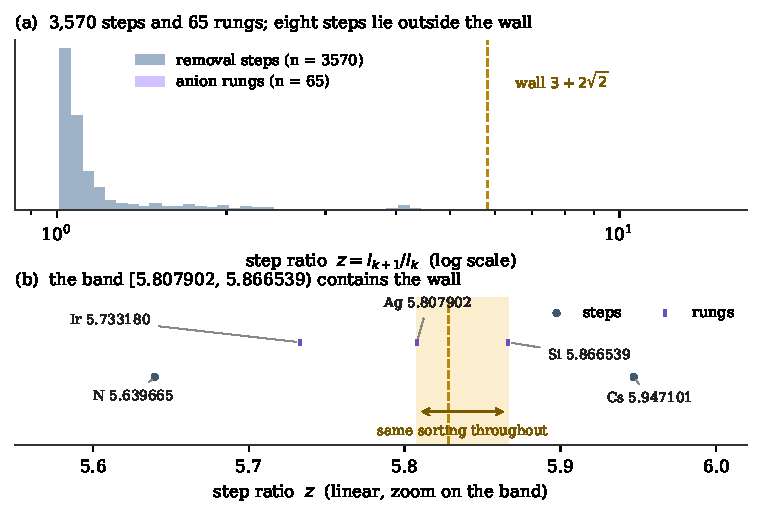
\includegraphics[width=\textwidth]{fig-band.pdf}
\caption{(a) All $3{,}570$ removal steps and 65 anion rungs of the baseline archive, on a
logarithmic ratio axis. The dashed line is the wall $\W$. (b) A linear zoom: the largest step
inside the wall (nitrogen, $5.639665$), the largest anion rung inside (silver, $5.807902$), the
wall, the smallest rung outside (silicon, $5.866539$) and the nearest step outside (caesium,
$5.947101$). Every cutoff in the shaded band classifies all $3{,}570$ steps identically. Drawn by
\texttt{scripts/band\_figure.py} from the shipped archive; no value is typed in.}
\label{fig:band}
\end{figure}

Order the $3{,}570$ baseline step ratios. The largest inside the wall is $5.639665$ (nitrogen,
$k=5$) and the smallest outside is $5.947101$ (caesium, $k=1$). Every cutoff in that interval
classifies all $3{,}570$ steps identically, and $\W=5.828427$ lies inside it. Adding the 65 anion
rungs narrows the interval to $[5.807902,5.866539)$---silver's rung the largest inside, silicon's
the smallest outside---which still contains the wall (Figure~\ref{fig:band}). (Measured:
\texttt{scripts/atlas\_census.py}.)

Nor do the aggregate counts rescue it. The $91{,}768$ and $91{,}638$ are deterministic functions
of the cutoff: at $c=5.85$, inside the band, the per-step classification is unchanged, still eight
outside and all core openings, but the crossing count falls to $91{,}616$ and the accumulated-only
count to $91{,}486$. The point is not that a computed quantity is never evidence; it is that these
counts have no independently measured target in the archive, so reproducing their published
values cannot select the cutoff. The raw endpoint ratios are cutoff-independent; which
compositions count as accumulated-only is not.

\subsection{A shape comparison}

The table also reports that reading each element's first eight steps on other shapes---triangle,
square, diamond, hexagon---groups elements by column far better than the raw energies do. On the
archive's 77-element comparison the scores are circle 53, diamond 52, cube 48, simplex 60 and raw
energies 4, with simplex numerically highest, a simplex-minus-circle gap of 7 of 77. The scoring
target and the evaluation population are fixed by that comparison and nothing beyond it is
inferred. (Measured: \texttt{scripts/shapes\_recall.py}.) The table's further claim that no shape
beats the circle by more than its bootstrap spread is not reproducible: no resampling unit,
replicate count, seed or spread is shipped.

\section{Reversal, sign, and what the wall cannot see}

Reversal sends $z\mapsto 1/z$ and $\G\mapsto-\G$, so any readout factoring through $\G^2$ cannot
distinguish a ratio from its reciprocal or the two branches of the wall. Two statements must be
kept apart here:
\begin{itemize}
\item a single ratio fixed by reversal has $z=1$ and $\G=0$, and is at neither branch;
\item a ladder fixed by reversal as a sequence---palindromic readings---need not have $\G=0$
  anywhere. The readings $1,W,1$ with $W=\W$ are unchanged by reversal and both of their steps are
  exactly at the wall.
\end{itemize}
The first is proved (\texttt{unified/Bridge/Chirality.lean},
\texttt{mirror\_fixed\_iff\_gam\_eq\_zero}). The second is the reason the distinction has to be
made in words; an earlier version of this material conflated them.

What the wall hides is the sign. Each branch has nonzero $\G$, and a $\G^2$ readout reports the
same number at $+\G$ and $-\G$. That is blindness to the sign of one coordinate and it is all that
is proved; $\G$ itself and $\log z$ are computed throughout the papers and are reversal-sensitive.
No further notion of chirality is formalised here.

The same elementary argument---an invariant odd under an involution vanishes on the fixed locus---
occurs in the other developments: a chiral pairing $STS^{-1}=-T$ pairs the spectrum and kills odd
moments, and $\theta(\text{mirror}\,K)=-\theta(K)$ makes $\theta$ vanish on amphichiral knots. It
is an analogy among proofs, not a compiled three-way interface. What is proved is the generic
lemma, an abstract $\theta$ schema whose $K$, mirror and $\theta$ are arbitrary, and the LoopWall
reversal identity; the Dirac spectral theorem is a separate argument and no knot invariant is
formalised. (Proved: \texttt{odd\_involution\_vanishes},
\texttt{theta\_vanishes\_on\_amphichiral}; not compiled as instances: Dirac, knots.)

The lemma gives one direction only. Over all $12{,}965$ prime knots through 13 crossings, KnotInfo
release 2026.11.2 has 78 amphicheiral (47 negative, 30 fully, 1 positive) and the name set is
identical to the 78 with $\theta=0$; there are none at 11 or at 13 crossings. That is a complete
finite verification and still not a proof of the converse, which is a statement about all knots. A
single odd function vanishing away from its fixed locus---$x^3-x$ at $x=1$---shows oddness alone
can never yield the converse. (Measured: \texttt{scripts/knot\_census.py} over two shipped lists.
Proved: \texttt{odd\_does\_not\_imply\_converse}. Open: the converse.)

\section{What is not established}

The negative results are part of the content, and they delimit the positive ones.
\begin{enumerate}[label=\arabic*.,leftmargin=2em]
\item Composition does not select the ledger readout. Evenness, vanishing at zero balance and
  append-additivity of a channel sum leave both the log ledger and the $\G^2$ readout admissible;
  selection needs additivity of a determinant readout plus regularity. (Proved:
  \texttt{append\_additivity\_alone\_does\_not\_select\_ledger};
  \texttt{CompositionBridge.eq\_const\_mul\_log\_of\_append\_additive}.)
\item Twelve statements transcribed from earlier prose are false as written and are kept as
  refutation theorems beside their corrected forms. (Proved: \texttt{FalseControls/};
  \texttt{LIMITATIONS.md}.)
\item The predictive quotient of a peel ladder is one-dimensional in the scalar present-reading
  model, and model-dependent rather than intrinsic: other linearisations of the same ladder
  separate the wall, and one changes dimension at $z=1$ instead. (Proved:
  \texttt{Bridge/Quotient.lean}; \texttt{Found/PredictivePeel.lean}.)
\item The block determinant identity is local: $1-\G^2=4\det p$ holds for one two-channel block;
  the composition bridge's \texttt{blockDet} is a product over blocks and equals $(1-\G^2)^n$. Two
  wall blocks give $1/4$, not $1/2$. (Proved: \texttt{Bridge/Reflection.lean};
  \texttt{Found/WallReadout.lean}.)
\item Perfect reflection is unattained: $\det p=0$ corresponds to $|\G|=1$, and for a positive
  ratio $|\G|<1$ strictly. (Proved: \texttt{Found/WallReadout.lean}.)
\end{enumerate}
These are not evidence for the positive statements. Assurance for each positive statement comes
separately, from its cited proof or its reproducible measurement; the corrigenda neither add to
that nor substitute for it.

\section{Prior art}\label{sec:prior}

Riccati equations for nonuniform transmission lines were standard long before this work. Pierce
gave the impedance Riccati equation and its uniform-line tanh solution in 1943 \cite{pierce};
Walker and Wax gave the voltage-reflection form in 1946 \cite{walkerwax}. The particular solution
$\G=\tanh(\omega t/2)$ follows from DLMF 4.34.3 with 4.35.12 \cite{dlmf} and needs no
transmission-line attribution. The identity \eqref{eq:smith} is DLMF 4.37.24. The addition law is
DLMF 4.35.3, which is also the relativistic velocity law in the tangent-half-angle variable. The
continued-fraction step matrix and its recurrence are standard (DLMF 1.12(ii); Paydon and Wall
\cite{paydonwall}; Kisil \cite{kisil}). The predictive quotient is the observability quotient of
linear systems theory. None of this is claimed as new.

What this paper offers is not an algebra and not a criterion:
\begin{enumerate}[label=(\roman*)]
\item a proof-level synthesis of four named works by this author, with the duplicate repository
  proofs kept and their interfaces stated as theorems---an integration of my own repositories, not
  a new algebraic object. The four, with versions: the loop-wall development in this repository;
  \emph{The Dirac Time of the Gigantefermion} \cite{dirac}; \emph{VOTKP: The Vector of Traits Kept
  under Peeling}, v2.9 \cite{votkp}; and the Ramanujan-faces session record of 13--15 November
  2026. The periodic table v2.2 supplies the data layer;
\item the application to removal-step ladders of the elementary product/log and mean bounds, with
  the archive counts and their Lean formalisation;
\item the restatement in peel notation of the eigenvalues of the standard continued-fraction
  matrix: with $r=x/(2n-1)$, $z_n=\exp(2\operatorname{asinh}r)$ and
  $\G_n=\tanh(\operatorname{asinh}r)=x/\sqrt{x^2+(2n-1)^2}$, whence $\G_n^2=\tfrac12$ exactly when
  $2n-1=x$. I have not located this displayed peel formulation elsewhere and claim only the
  formulation and the odd-$x$ observation;
\item the itemised corrigenda, and the computation that this archive leaves an interval of cutoffs
  with identical per-step classifications while yielding different aggregate counts inside it.
  Both are repository- and archive-specific.
\end{enumerate}
The last is the most defensible contribution and the least exciting: a checked statement of what
the evidence does not show.

\section{Scope}\label{sec:scope}

No physical mechanism is derived. No Hamiltonian, force, optical constant or ionisation energy is
produced, and the one rate identification in Section~\ref{sec:where} is marked as an
identification. No predictive power over chemistry is claimed: the body sorts ratios that were
already measured and has not predicted one that was not. The wall value is not selected from data
(Section~\ref{sec:band}). The knot converse is open. Theta is not formalised, and neither is the
continued fraction. The developments were not one programme; the unification is retrospective.

A reader who wants the shortest true description: four developments share a coordinate, three
interfaces between them are compiled, one table is consistent with the coordinate's constant but
cannot select it, and the negative results are the part most likely to be confirmed by someone
else's checking.

\appendix
\section{The ledger}\label{app:ledger}

Every claim, with status and reproducer. ``proved${}^*$'' means proved about definitions this tree
introduces, not about the external object the section names. Scripts are in \texttt{scripts/}.

{\scriptsize
\begin{longtable}{>{\raggedright\arraybackslash}p{0.53\textwidth}%
                  >{\raggedright\arraybackslash}p{0.11\textwidth}%
                  >{\raggedright\arraybackslash}p{0.28\textwidth}}
\toprule
\textbf{claim} & \textbf{status} & \textbf{reproducer}\\
\midrule
\endhead
\multicolumn{3}{l}{\emph{proved}}\\
\midrule
$\G=\tanh(\log z/2)$ & proved & \texttt{Ledger.lean} / \texttt{Smith.lean}\\
$z=(1+\G)/(1-\G)$ & proved & \texttt{Ledger.lean}, \texttt{inverse\_gam}\\
$\G(1/z)=-\G(z)$, squares equal & proved & \texttt{gam\_reverse}, \texttt{gam\_sq\_reverse}\\
$\G^2=\tfrac12$ iff $z=3\pm2\sqrt2$ & proved & \texttt{Wall.lean}, \texttt{wall\_eq\_iff}\\
wall ledger $=\pm2\log(1+\sqrt2)$ & proved & \texttt{Bridge/Reflection}\\
window exceeds $W$ iff sum rapidity $>\log W$ & proved & \texttt{Bridge/Composition}\\
two steps at $5/2$ cross ($25/4$) & proved & \texttt{two\_halves\_cross}\\
geometric mean of inside steps inside & proved & \texttt{geomean\_lt\_wall}\\
$\G_n=x/\sqrt{x^2+(2n-1)^2}$ & proved${}^*$ & \texttt{Bridge/Faces}\\
a face is on the wall iff $2n-1=x$ & proved${}^*$ & \texttt{faceGamma\_sq\_eq\_half\_iff\_odd}\\
Brouncker $z_1=\W$ & proved${}^*$ & \texttt{brouncker\_first\_face}\\
odd invariant vanishes on fixed locus & proved & \texttt{Bridge/Chirality}\\
oddness does not give the converse & proved & \texttt{odd\_does\_not\_imply\_converse}\\
$\mu_j-\mu_k=\dot\tau(E_j-E_k)$ & proved & \texttt{DiracTime/CommonClock}\\
$\omega=\mu_j-\mu_k$, the peel rate & --- & model identification\\
$|\delta|\tau_{\text{wall}}=\log\W$ & proved & \texttt{Found/CommonClock}\\
descent specialises to the peel ledger & proved & \texttt{tanh\_ledger\_descent}\\
predictive quotient, two proofs agree & proved & \texttt{unseen\_eq\_unobservable}\\
readout non-selection (6.1) & proved & \texttt{append\_additivity\_alone\_\dots}\\
peel dimension one, scalar model (6.3) & proved & \texttt{Bridge/Quotient}\\
\dots and model-dependent elsewhere (6.3) & proved & \texttt{Found/PredictivePeel}\\
$1-\G^2=4\det p$, one block (6.4) & proved & \texttt{Bridge/Reflection}\\
$\texttt{blockDet}=(1-\G^2)^n$ (6.4) & proved & \texttt{Found/WallReadout}\\
perfect reflection is unattained (6.5) & proved & \texttt{Found/WallReadout}\\
twelve prose statements false (6.2) & proved & \texttt{FalseControls/}, \texttt{LIMITATIONS.md}\\
\midrule
\multicolumn{3}{l}{\emph{measured}}\\
\midrule
$3{,}570$ steps; 8 outside; all core openings & measured & \texttt{atlas\_census.py}\\
305/305 core records satisfy $k=Z-N$ & measured & \texttt{atlas\_census.py}\\
65 rungs; 53 outside & measured & \texttt{atlas\_census.py}\\
83 maxima $=78$ He $+2$ Ne $+1+1+1$ & measured & \texttt{atlas\_census.py}\\
118 elements; $5{,}714$ steps & measured & \texttt{atlas\_census.py}\\
$183{,}770\,/\,91{,}768\,/\,91{,}638\,/\,0$ & measured & \texttt{atlas\_census.py}\\
main triple invariant to ratio convention & measured & \texttt{atlas\_census.py}\\
control $191{,}817\,/\,98{,}572\,/\,98{,}442$ & measured & \texttt{atlas\_census.py}\\
control $191{,}817\,/\,95{,}569\,/\,95{,}439$ & measured & \texttt{atlas\_census.py}\\
130 crossing windows contain an outside step & measured & \texttt{atlas\_census.py}\\
$99.86$ per cent & measured & \texttt{atlas\_census.py}\\
$183{,}081$ usable; 689 missing; 0 upper & measured & \texttt{atlas\_census.py}\\
$4.76566745$ (Li); $3.15005083$ (B) & measured & \texttt{atlas\_census.py}\\
band $[5.639665,5.947101)$ & measured & \texttt{atlas\_census.py}\\
combined band $[5.807902,5.866539)$ & measured & \texttt{atlas\_census.py}\\
$91{,}486$ windows at $c=5.85$ & measured & \texttt{atlas\_census.py}, checker\\
shapes $53/52/48/60$ of 77; raw 4/77 & measured & \texttt{shapes\_recall.py}\\
simplex $-$ circle $=7/77$ & measured & \texttt{shapes\_recall.py}\\
uniform chance $0.044429254956$ & measured & \texttt{shapes\_recall.py}\\
$12{,}965$ knots; $78=47+30+1$; 0 at 11,13 & measured & \texttt{knot\_census.py}\\
KnotInfo names $=$ theta-zero names & measured & \texttt{knot\_census.py}\\
Ramanujan finite values at $N=6400$ & measured & \texttt{ramanujan\_faces.py}\\
attenuation spread $\le5$ per cent & measured & \texttt{ramanujan\_faces.py}\\
angle table (eight fractions) & measured & \texttt{ramanujan\_faces.py}\\
$1{,}594$ declarations, $1{,}591$ build-covered & measured & \texttt{build\_unified.py -{}-count}\\
93 modules in this material (95 in the build) & measured & \texttt{build\_unified.py}\\
65 audited declarations ($39+26$) & measured & \texttt{Bridge/Audit.lean}, \texttt{AuditAll.lean}\\
\midrule
\multicolumn{3}{l}{\emph{open, or not reproducible here}}\\
\midrule
the limits $4/\pi^2$ and $1/4$ & open & finite evidence only\\
the $N^{-x}$ error law & open & motivated, not derived\\
the fraction's terms \emph{are} these faces & --- & reading\\
bootstrap spread of the shape scores & --- & not shipped\\
a knot invariant ($\theta$) itself & --- & not formalised\\
the Dirac pairing as an instance of the generic lemma & --- & analogy among proofs\\
the lower wall branch in the composition criterion & open & stated for $W$ only\\
\bottomrule
\end{longtable}
}

\begin{thebibliography}{9}
\bibitem{pierce} J.~R. Pierce, ``A note on the transmission line equation in terms of
impedance'', \emph{Bell System Technical Journal} \textbf{22} (1943) 263--265.
\bibitem{walkerwax} L.~R. Walker and N.~Wax, ``Non-uniform transmission lines and reflection
coefficients'', \emph{Journal of Applied Physics} \textbf{17} (1946) 1043--1045.
\bibitem{dlmf} NIST \emph{Digital Library of Mathematical Functions},
\url{https://dlmf.nist.gov/}: eqs.~1.12(ii), 4.8.2, 4.34.3, 4.35.3, 4.35.12, 4.37.24.
\bibitem{paydonwall} W.~D. Paydon and H.~S. Wall, ``The continued fraction as a sequence of
linear transformations'', \emph{Duke Mathematical Journal} \textbf{9} (1942).
\bibitem{kisil} A.~V. Kisil, ``Remark on continued fractions, M\"obius transformations and
cycles'', \texttt{arXiv:1412.1457}, \S2.
\bibitem{dirac} J.~Beasley, \emph{The Dirac Time of the Gigantefermion}.
\href{https://doi.org/10.5281/zenodo.22978630}{doi:10.5281/zenodo.22978630}.
\bibitem{votkp} J.~Beasley, \emph{VOTKP: The Vector of Traits Kept under Peeling}, v2.9.
\href{https://doi.org/10.5281/zenodo.23340757}{doi:10.5281/zenodo.23340757}.
\bibitem{knotinfo} C.~Livingston and A.~H. Moore, \emph{KnotInfo: Table of Knot Invariants},
\url{https://knotinfo.org/}, release 2026.11.2.
\end{thebibliography}

\end{document}
